\documentclass[tikz,border=3mm]{standalone}
\usepackage{tikz}
\usetikzlibrary{calc}
\begin{document}
% TikZ 1
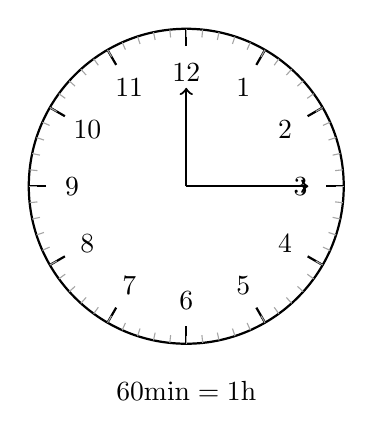
\begin{tikzpicture}[scale=1]
\draw[thick] (0,0) circle (2);
\foreach \n in {1,...,12}{
  \draw[thick] ({90-30*\n}:1.78)--({90-30*\n}:2);
  \node at ({90-30*\n}:1.45) {$\n$};
}
\foreach \n in {0,...,59}{
  \draw[gray!70] ({90-6*\n}:1.9)--({90-6*\n}:2);
}
\draw[thick,->] (0,0)--(90:1.25);
\draw[thick,->] (0,0)--(0:1.55);
\node[below] at (0,-2.35) {$60\mathrm{min} = 1\mathrm{h}$};
\end{tikzpicture}
\hspace{1cm}
% TikZ 2
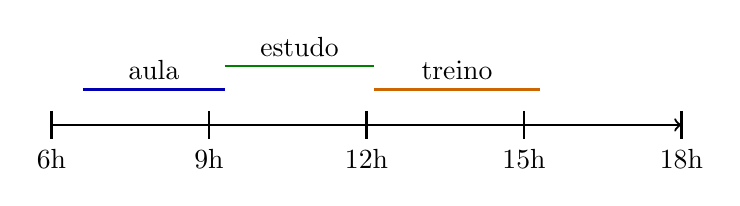
\begin{tikzpicture}[scale=1]
\draw[thick,->] (0,0)--(8,0);
\foreach \x/\ticklabel in {0/6\mathrm{h},2/9\mathrm{h},4/12\mathrm{h},6/15\mathrm{h},8/18\mathrm{h}}{
  \draw[thick] (\x,.18)--(\x,-.18);
  \node[below] at (\x,-.18) {$\ticklabel$};
}
\draw[blue!70!black,thick] (.4,.45)--(2.2,.45);
\draw[green!50!black,thick] (2.2,.75)--(4.1,.75);
\draw[orange!80!black,thick] (4.1,.45)--(6.2,.45);
\node[above] at (1.3,.45) {aula};
\node[above] at (3.15,.75) {estudo};
\node[above] at (5.15,.45) {treino};
\end{tikzpicture}

\vspace{1cm}

% TikZ 3
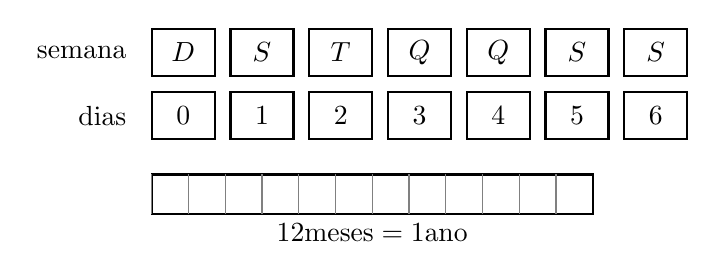
\begin{tikzpicture}[scale=1]
\foreach \i/\weekday in {0/D,1/S,2/T,3/Q,4/Q,5/S,6/S}{
  \draw[thick] (\i,1.4) rectangle +(0.8,0.6);
  \node at (\i+.4,1.7) {$\weekday$};
}
\foreach \i in {0,...,6}{
  \draw[thick] (\i,.6) rectangle +(0.8,0.6);
  \node at (\i+.4,.9) {$\i$};
}
\node[left] at (-.2,1.7) {semana};
\node[left] at (-.2,.9) {dias};
\draw[thick] (0,-.35) rectangle (5.6,.15);
\foreach \m in {0,...,11}{
  \draw[gray] ({\m*5.6/12},-.35)--({\m*5.6/12},.15);
}
\node[below] at (2.8,-.35) {$12\mathrm{meses} = 1\mathrm{ano}$};
\end{tikzpicture}
\hspace{1cm}
% TikZ 4
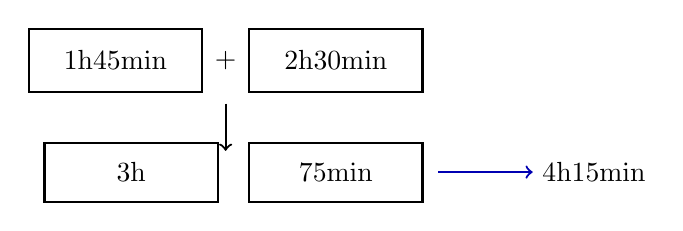
\begin{tikzpicture}[scale=1]
\draw[thick] (0,1.4) rectangle (2.2,2.2);
\node at (1.1,1.8) {$1\mathrm{h}45\mathrm{min}$};
\draw[thick] (2.8,1.4) rectangle (5,2.2);
\node at (3.9,1.8) {$2\mathrm{h}30\mathrm{min}$};
\node at (2.5,1.8) {$+$};
\draw[->,thick] (2.5,1.25)--(2.5,.65);
\draw[thick] (.2,0) rectangle (2.4,.75);
\node at (1.3,.38) {$3\mathrm{h}$};
\draw[thick] (2.8,0) rectangle (5,.75);
\node at (3.9,.38) {$75\mathrm{min}$};
\draw[->,blue!70!black,thick] (5.2,.38)--(6.4,.38);
\node[right] at (6.4,.38) {$4\mathrm{h}15\mathrm{min}$};
\end{tikzpicture}
\end{document}
